\section{Conjugate Gradients (5/5 Points)}

\subsection{Task 2a - A CUDA Kernel for the Matrix-Vector Product (1 Point)}
Below the listing with the relevant code chunk for Task 2a.
\begin{lstlisting}[language=C++, title=C++ Cuda Code for 1a Kernel]
__global__ void CUDA_csr_matvec_product(size_t N, int *csr_rowoffsets, int *csr_colindices, double *csr_values, double *x, double *y)
{
  for (int row = blockDim.x * blockIdx.x + threadIdx.x; row < N; row += gridDim.x * blockDim.x)
  {
    double val = 0;
    for (int jj = csr_rowoffsets[row]; jj < csr_rowoffsets[row + 1]; ++jj)
    {
      val += csr_values[jj] * x[csr_colindices[jj]];
    }
    y[row] = val;
  }
}
\end{lstlisting}



\pagebreak


\subsection{Task 2b - CUDA Kernels for Vector Operations (2 Points)}
Below the listings with the relevant code chunks for Task 2b.
\begin{lstlisting}[language=C++, title=C++ Cuda Code for 1a Kernel]
__global__ void CUDA_dot_product(int N, double *x, double *y, double *result)
{
  __shared__ double shared_mem[1024];
  double dot = 0;
  for (int i = blockIdx.x * blockDim.x + threadIdx.x; i < N; i += blockDim.x * gridDim.x)
  {
    dot += x[i] * y[i];
  }
  shared_mem[threadIdx.x] = dot;
  for (int k = blockDim.x / 2; k > 0; k /= 2)
  {
    __syncthreads();
    if (threadIdx.x < k)
    {
      shared_mem[threadIdx.x] += shared_mem[threadIdx.x + k];
    }
  }
  if (threadIdx.x == 0)
  {
    atomicAdd(result, shared_mem[0]);
  }
}

__global__ void vectorAdd_Kernel_7(int N, double *x, double *y, double a)
{
  for (int i = blockIdx.x * blockDim.x + threadIdx.x; i < N; i += blockDim.x * gridDim.x)
  {
    x[i] += a * y[i];
  }
}

__global__ void vectorAdd_Kernel_8(int N, double *x, double *y, double a)
{
  for (int i = blockIdx.x * blockDim.x + threadIdx.x; i < N; i += blockDim.x * gridDim.x)
  {
    x[i] -= a * y[i];
  }
}

__global__ void vectorAdd_Kernel_12(int N, double *x, double *y, double a)
{
  for (int i = blockIdx.x * blockDim.x + threadIdx.x; i < N; i += blockDim.x * gridDim.x)
  {
    x[i] = y[i] + a * x[i];
  }
}
\end{lstlisting}

\pagebreak

\subsection{Task 2c - Convergence Behaviour of CUDA Cojungate Gradient (1 Point)}
Plots for Task 2!
  \begin{figure}[h]
    \begin{center}
      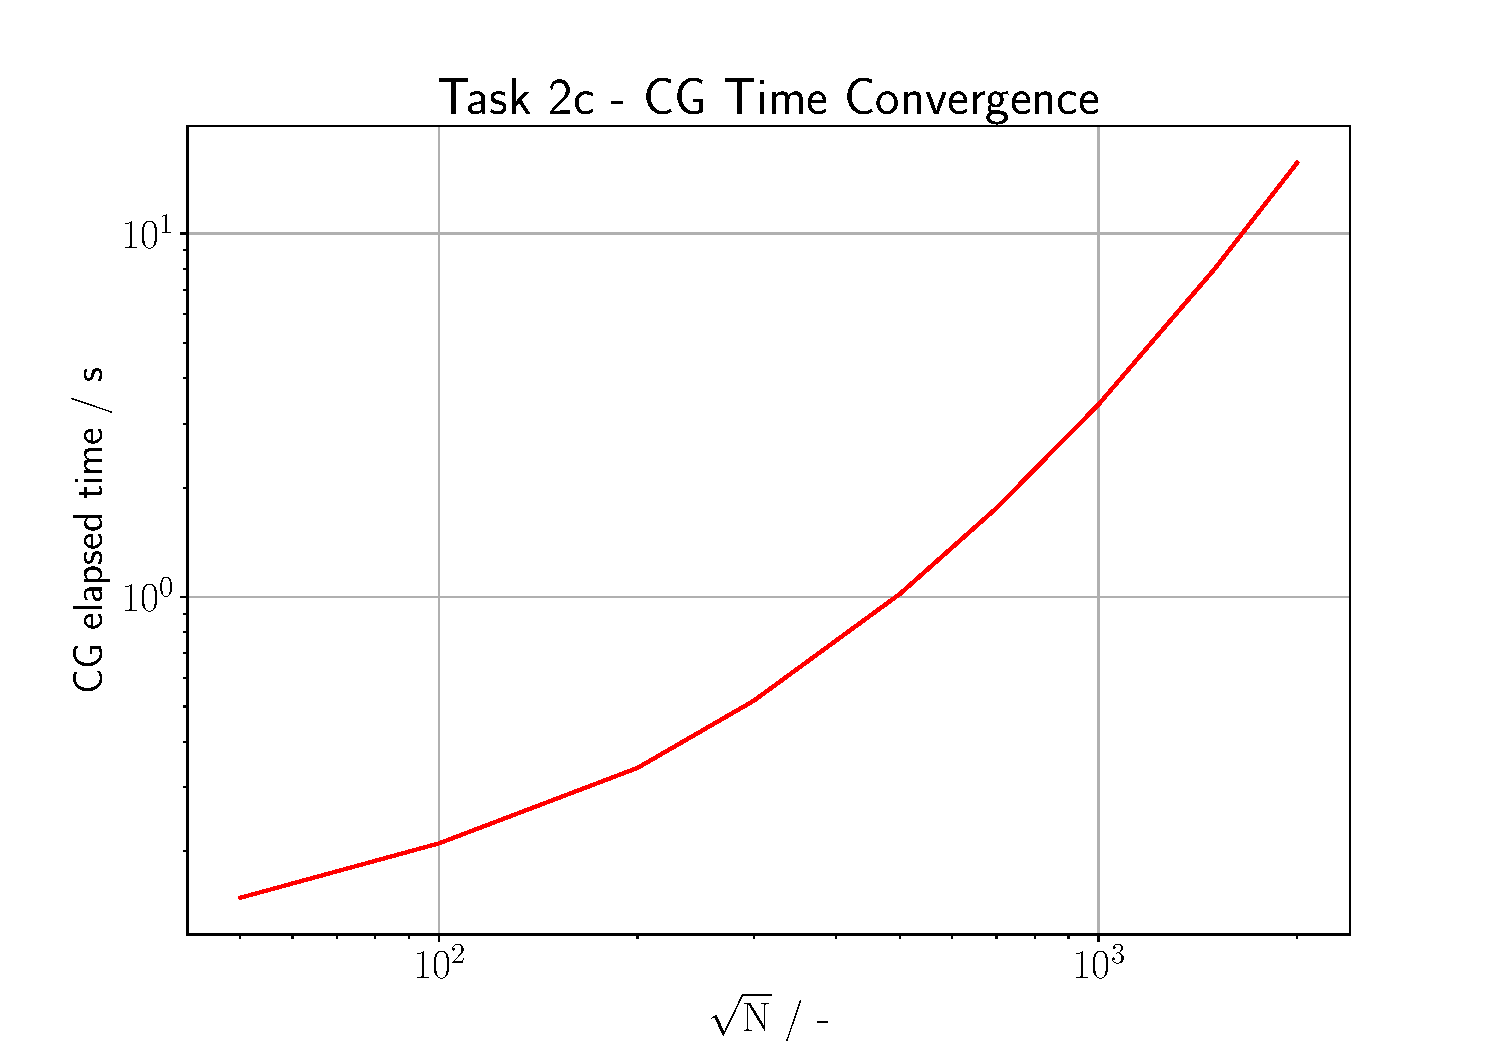
\includegraphics[width= 0.7\linewidth]{figures/task_2_c_1.pdf}
      \caption{Partial Results for Task 2c}
      \label{label_2c1_figure}
    \end{center}
  \end{figure}

  \begin{figure}[h]
    \begin{center}
      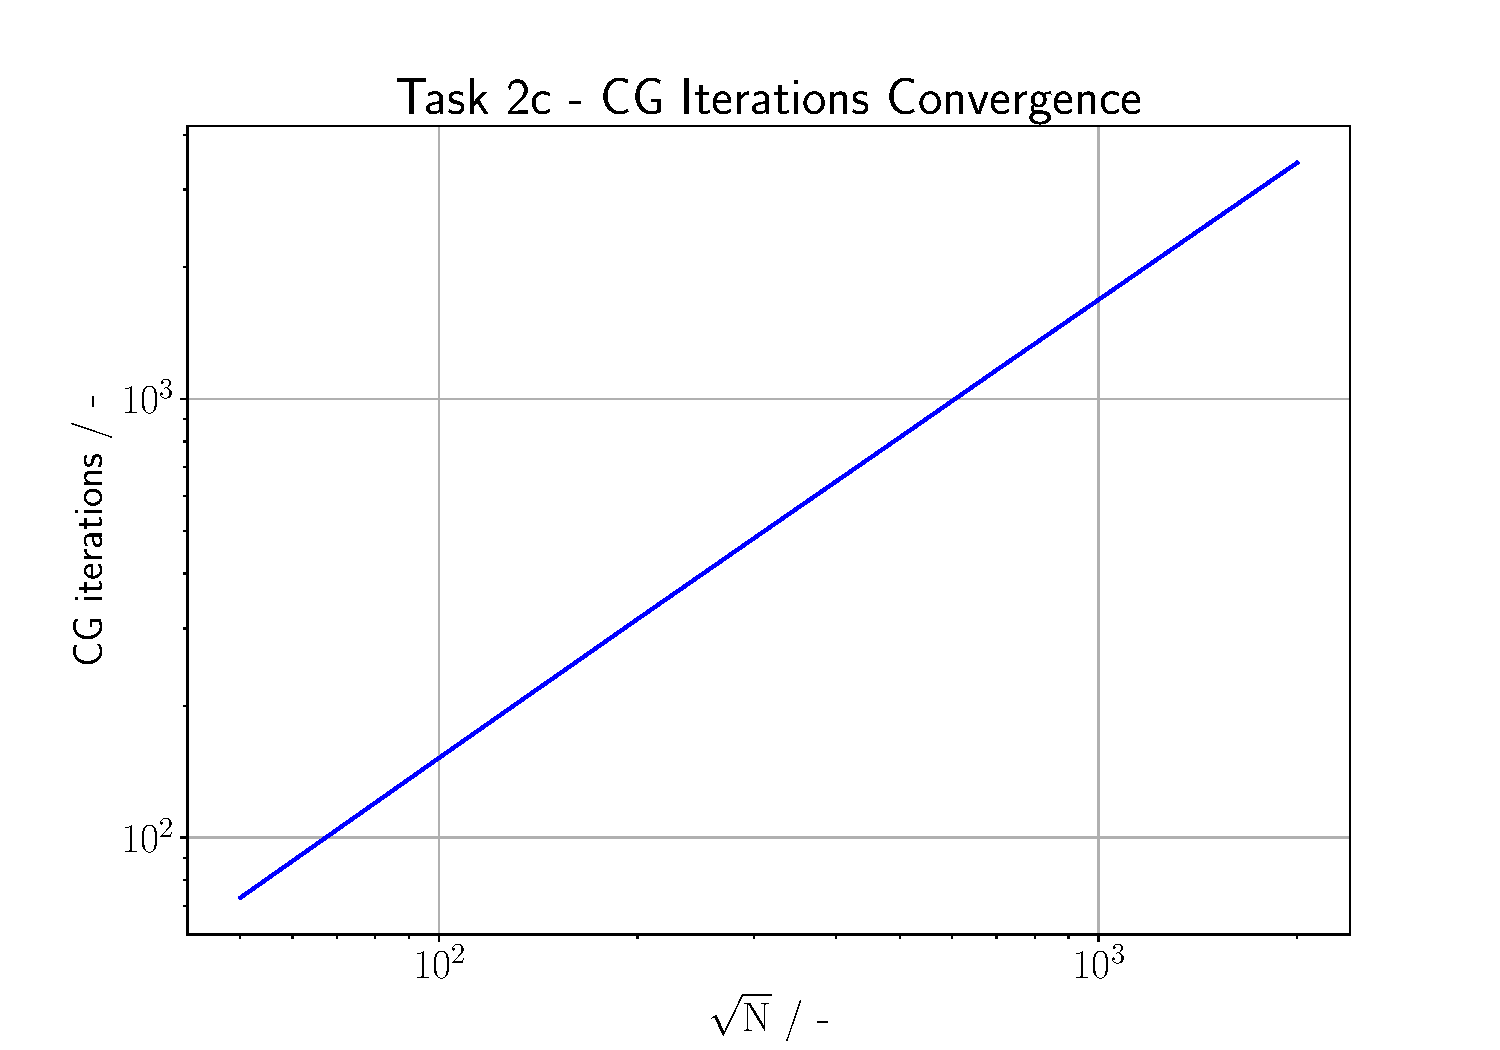
\includegraphics[width= 0.7\linewidth]{figures/task_2_c_2.pdf}
      \caption{Partial Results for Task 2c}
      \label{label_2c2_figure}
    \end{center}
  \end{figure}

\pagebreak

\subsection{Task 2d - Which Parts are worthwile optimizing? (1 Point)}
The addition kernels seem worthwhile optimizing!
\begin{lstlisting}[language=C++, title=C++ Console output for sqrt(N) = 2000]
CG converged after 3454 iterations.
CUDA_csr_matvec_product: 0.000002
CUDA_dot_product: 0.000253
vectorAdd_Kernel_7: 0.000288
vectorAdd_Kernel_8: 0.000291
vectorAdd_Kernel_12: 0.000288
Relative residual norm: 1.56973e-07 (should be smaller than 1e-6)
t = 16.063496
  \end{lstlisting}

\pagebreak